% Chapter 3 - Description of problem

\chapter{Application of Nek5000} % Main chapter title

\label{problem} % Change X to a consecutive number; for referencing this chapter elsewhere, use \ref{ChapterX}

\lhead{Chapter 3. \emph{application of Nek}} % Change X to a consecutive number; this is for the header on each page - perhaps a shortened title

%----------------------------------------------------------------------------------------
%	SECTION 1
%----------------------------------------------------------------------------------------
\colorbox{yellow}{Some introduction about flow solvers in general and how Nek differs from these}
There are many numerical solvers for turbulent flows available on the market.
From large commercial softwares such as Fluent which runs as a 
black-box solver, to full open-source codes such as nek5000 and openFOAM. 
The solvers can vary both in the fundamental numerical method (FV,FD,FEM,SEM) 
the time-step method (Fractional Step, Poisson pressure, Uzawa) 
and the type of simulation (RANS,LES,DNS).

%An example is waterflow in a channel, which would be the practical problem. 
%The mathematical formulation would be the incompressible N-S eq, 
%with LES dynamical SGS. The mesh could consist of tetrahedros or hexahedrons.
%The simulation is the performed on some cluster before the 
%wanted data in some sub-domain is visualized and presented. 

\section{Nek5000 Basics }
Nek5000 is a turbulent flow solver developed mainly by Paul Fischer
and has through the past 20 years had several contributours. 
It is an open-source code applicable to many different types of flow 
and it has been put a lot of effort into making the code as parallelizable as possible.
With SEM as the numerical method applied it is possible to obtain extremely accurate results.  

nek5000 has its own mesh-generator for generating simpler geometries and it is also implemented the possibility to integrate CUBIT mesh 
files. A common starting point for simulating turbulent flow is a geometry given by a CAD-file,
without any functions to describe the boundaries.
The possibility to make a mesh through a visual gui is provided through for instance ICEM.
This mesh can then later be transformed to the inputfile required by nek5000. 

So far nek5000 has supported three automatic routine for generating curved edges;
circles in 2-D geometries, spherical shell elements and a general 2nd degree interpolation.
Further manipulation of the element edges is left to the user to define manually
for each particular problem. One of the objectives of this thesis is to make Nek5000 more
user-friendly and create automatic routines to handle complex geometry.

In order to get a quick overview of the framework in Nek a short list of the main steps
are stated in the list below 
%
\begin{enumerate}
    \item \emph{Initialize} 
    \subitem Reading mesh and parameters from user, generating GLL-points, and defining
        the values needed to perform the simulations. PRESSURE SOLV INIT ??? 
    \item \emph{solve}
     \subitem Solving for each timestep, depending on the problem solvers for flow,temperature 
     and other scalars will be performed. The user is free to choose different solvers which 
     will be discussed later.
 \item \emph{post-processing}
     \subitem Writing statistics and other user-specified parameters to file.
\end{enumerate}
%
Nek provides a basic tool for generation of mesh. For more complex geometries this tool cannot compare with more visualized-based softwares 
such as ICEM from ANSYS which exports mesh to several numerical solvers such as Fluent and nastran.
It is therefore very useful to have an automatic way of converting a mesh created in ICEM to the format required by nek5000. 
In order for nek to run optimally the elements should be as homogenous and as similar to the reference element as possible. 
It is therefore of great interest to be able to propagate curved geometries into the neighbour-elements in order to have a smooth as 
possible transition from a boundary with high curvature.

\subsection{Incompressible N-S solvers in Nek}
A Convection-Diffusion problem can be stated as 
\begin{align}
    M\frac{du}{dt} = Au-Cu+Mf
    \label{eq:conv-diff}
\end{align}
% 
Where $M$ and $A$ is the mass, and stiffness matrix, $f$ is the loading function and $C$ is 
the matrix corresponding to the convective term. The non-linearity is represented in the 
convective term since $C$ is dependent of $u$.
The time-derivative is discretized by a Backward difference (BDFk) scheme using solutions 
from the $k$ previous steps to extrapolate the current value. In order to gain stability 
an implicit scheme is chosen and the resulting eguation is given as 
%
OIFS ???
---------- CHECK MAKEF IN NAVIER1.F ----------------- 
\begin{align}
    \sum_{j=0}^{k}\frac{b_j}{\Delta t}Mu^{n-j+1} = Au^{n+1}-Cu^{n+1}+Mf^{n+1}
    \label{eq:conv-diff2}
\end{align}
% 
By extrapolating the convective term from the $k$ previously calculated steps the equation 
simplifies to 
%
\begin{align}
   \frac{b_0}{\Delta t}Mu^{n+1} \sum_{j=1}^{k}\frac{b_j}{\Delta t}Mu^{n-j+1} 
   = Au^{n+1}-\sum_{j=1}^{k}a_jCu^{n-j+1}+Mf^{n+1}
    \label{eq:conv-diff3}
\end{align}
% 
and finally by moving all the explicit terms to the rhs the equation left to solve is given as 
%
\begin{align}
   (\frac{b_0}{\Delta t}M-A)u^{n+1} 
   = -\sum_{j=1}^{k}(\frac{b_j}{\Delta t}M-a_jC)u^{n-j+1}+Mf^{n+1}
    \label{eq:conv-diff4}
\end{align}
% 
Notice from Section~\ref{theory} that this is equivalent to the matrix formulation of 
the Helmholtz equation.



\subsection{Nek5000 for complex geometries}

\section{Case 1: Gas dispersion in a simplified urban area}
The problem investigated in this work is gas dispersion of neutral gas in a velocity field through four cubic blocks.
Similar simulations have been done in CDP and Fluent which are compared to data from a wind-tunnel experiment performed by ALAN.
\begin{itemize}
	\item Description of problem and domain
	\item mesh and fluent/CDP mesh
\end{itemize}

\section{Case 2: Drag and lift on a cylinder}
Descrition of problem\ldots
Descrition of implementation approach in Nek\ldots

\section{Advances in the mesh-generation routine}
The routine xyzarc:

The gordon hall algorithm was already implemented as a function in Nek, with the gll-points,plynomial degree and some initial 
coordinates to the element. The algorithm creates a distribution of the internal gll-points in each element. 
If the element consists of linear edges the only necessary input are the vertices, but by specifying the points on edges and faces
the algorithm creates a logical distribution of the internal GLL-points to a deformed element. 

The curved edge is specified in the .rea file and the routine genxyz() processes the input of each edge. 
By specifying the radius and the circle center genxyz calls the routine xyzarc() which performs the following algorithm;

    $a,b$ will be the two endnodes of the edge 
    $c$ will be the midnode, $s$ will be the arc length, $\theta$ will be the full angle of the circle sector, $cc$ is the center coordinates.
    $g$ will be the vector containing the GLL-points in $[-1,1]$. $r$ will be the radius.

	%/* Pseudo code */
%define interpolation algorithm 
%\textbf{\textbf{for}} each timestep \emph{T}
  %Read inflow
  %\textbf{for} each node \emph{N} and velocity component \emph{V} on inflow boundary 
    %\emph{V}(\emph{N}) = doInterpolation(N)
  %\textbf{endfor}
  %solve
%\textbf{endfor}
\begingroup
\fontsize{12pt}{14pt}
\begin{lstlisting}[escapechar=|]
 l = a-b                       # vector between the corner nodes
 c = (a+b)/2                   # midpoint location
 h = c-cc                      # height of the framed triangle
 |$\theta$| = arctan(abs(l)/2abs(h))    # half the angle of the circle sector
 s = r*|$\theta$|                       # arclength
 g' = g*|$\theta$|                      # angles to the gll-points on the circle-sector
 #---------- Finding the intersecting points ----------#
 #---- x on the line l, and extend x-cc to the arc ----#
 |\textbf{for}| k in range(lx1):          # For the number of nodes in one direction
    |$\alpha$| = h*tan(g'[k])           # Offset from the midpoint on l
    x = c-|$\alpha$|*l/abs(l)           # Actual coordinate on l
    m = x-cc                   # hypothenus of the imposed triangle
    edge(k) = cc+r*m/abs(m)    # final coordinate on the arc
\end{lstlisting}
\endgroup
These lines creates the wanted egde curved as a circle sector corresponding to the radius and circle center given.
The remaining operation is to call the gordon hall algorithm and create the internal GLL-points defined by the edges 
provided. The figure~\ref{fig:curvature} illustrates the geometry on which the algorithm is performed.
Notice that the algorithm assumes that the center is somewhere on the plane defined as all the 
points with equal distance to both $a$ and $b$.


\begin{figure}[h]
    \centering
    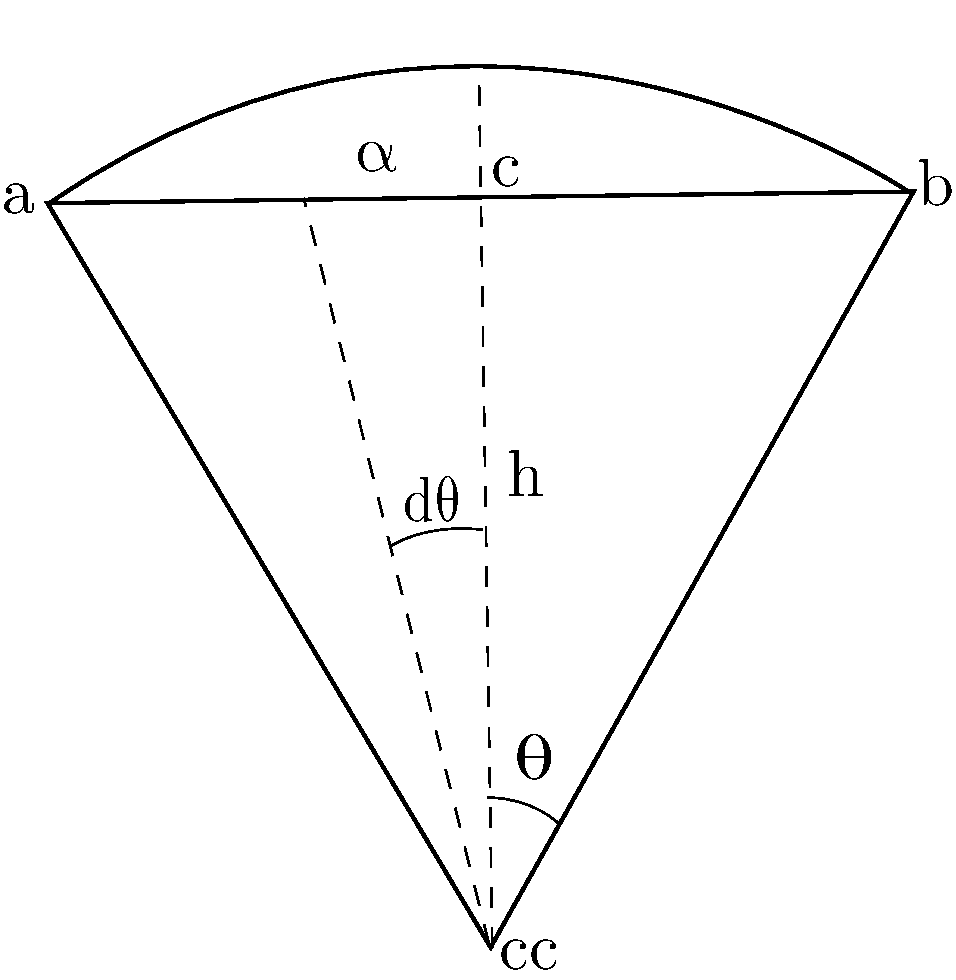
\includegraphics[width = 0.5\textwidth]{Figures/curvature.pdf}
    \caption{A sketch of the curved edge and the variables necessary to calculate the projection}
    \label{fig:curvature}
\end{figure}


\begin{itemize}
	\item initial script
	\item changes and modifications
	\item performance testing
	\item pitfalls
\end{itemize}
